\chapter{Turbulence Modelling} % Main chapter title
\label{Chapter2}

\section{Viscosity-Based Models}
Violeau et al. \parencite{VIOLEAU2002} were amongst the early pioneers who tried to incorporate a turbulence model in SPH. They came up with two techniques to tackle the problem of turbulence in a Lagrangian framework, which so far had been neglected till then in research, namely, the eddy viscosity model and a generalised Langevin model. For each of their techniques, they considered the following equation of state \ref{eq:violeau-eos}, continuity equation \ref{eq:violeau-continuity} and momentum equation \ref{eq:violeau-mom}, based on the work of \parencite{Monaghan1992}:

\begin{equation}
    P_i = \frac{\rho_0 c_s^2}{\gamma} \Bigg[ \bigg( \frac{\rho_i}{\rho_0} \bigg)^{\gamma} - 1 \Bigg]
    \label{eq:violeau-eos}
\end{equation}
\begin{equation}
    \LagDerivative{\rho_i} = \sum_j m_j \VIJ \cdot \DWIJ
    \label{eq:violeau-continuity}
\end{equation}
\begin{equation}
    \LagDerivative{\vect{v}_i} = \sum_j m_j \bigg( \frac{P_i}{\rho_i^2} + \frac{P_j}{\rho_j^2} + \Pi_{ij} \bigg) \DWIJ + \vect{F}_i
    \label{eq:violeau-mom}
\end{equation}

Where the viscous term is defined as:
\begin{equation}
    \Pi_{ij} = - \frac{16\nu}{\rho_i + \rho_j} \frac{\VIJ \cdot \RIJ}{\RtwoIJ + \MachineEpsilon^2} 
    \label{eq:violeau-diffusion-term}
\end{equation}

\subsection{Eddy Viscosity Model}
\label{sec:eddy-visc-model}

The eddy viscosity model was devised as a first-order closure model, which consisted of a relationship between the Reynolds stress tensor and the mean velocity gradients. Therefore, the momentum equation is similar to the momentum equation, except that the kinematic viscosity is replaced by the eddy viscosity $(\nu_t)$, and the velocities are Reynolds-averaged. In the SPH formalism, the diffusion term occurring is therefore defined as given in \ref{eq:violeau-turbulent-diffusion-term}, with the eddy viscosity defined according to \ref{eq:violeau-eddy-viscosity}.
\begin{equation}
    \Tilde{\Pi}_{ij} = -8 \frac{\nu_{t, i} + \nu_{t, j}}{\rho_i + \rho_j} \frac{\RAProp{\vect{v}}_{ij} \cdot \RIJ }{\RtwoIJ + \MachineEpsilon^2}
    \label{eq:violeau-turbulent-diffusion-term}
\end{equation}
\begin{equation}
    \nu_t = L_m^2 \FrobeniusNorm{\tensor{S}}
    \label{eq:violeau-eddy-viscosity}
\end{equation}

Where $\RAProp{\vect{v}}$ is Reynolds-averaged velocity, and $L_m$ refers to the mixing length scales. The SPH formulation for the mean velocity gradients are given in \ref{eq:violeau-mean-velocity-gradient}.

\begin{equation}
    \nabla \RAProp{\vect{v}}_i = - \frac{1}{\rho_i} \sum_j m_j \RAProp{\vect{v}}_{ij} \otimes \DWIJ
    \label{eq:violeau-mean-velocity-gradient}
\end{equation}

On simulating Poiseuille flow for a high Reynolds number case, the authors could show that the velocity profile showed only a slight discrepancy with theory, with the expected log-law profile near the walls \ref{fig:violeau2002-eddy-viscosity-result}. This indicated that the model is appropriate for turbulent mixing problems or for cases involving spatially-varying viscosity while restricted to shear flows.

\begin{figure}[h]
    \centering
    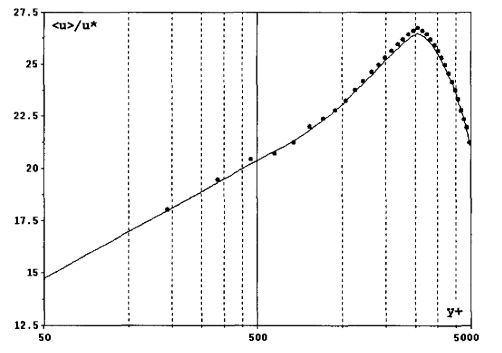
\includegraphics{Figures/research_papers/violeau2002-eddy-viscosity-result.png}
    \caption{Turbulent Poiseuille flow in a pipe $(Re = 64e3)$ modelled using the eddy viscosity model. Computed mean velocity profiles after $(t=1s)$ (solid circles), against theory (solid line). Ref: \parencite{VIOLEAU2002}}
    \label{fig:violeau2002-eddy-viscosity-result}
\end{figure}

\subsection{Generalized Langevin Model}
Violeau et al. also considered a stochastic approach, where the main idea is built on the concept of prescribing particle velocities as a random process, with properties fulfilling the theoretical turbulence hypotheses \parencite{pope1994lagrangi}. Hence, came about the Generalised Langevin model (GLM), where the particle acceleration is defined as:
\begin{equation}
    d\vect{v} = -\frac{1}{\rho} \nabla \RAProp{P} + \tensor{G}(\vect{v} - \RAProp{\vect{v}})dt + \sqrt{C_0 \epsilon dt}\vect{\xi}
    \label{eq:violeau-glm-particle-accel}
\end{equation}

Where $\Vec{\xi}$ is a random vector statistically non-correlated with velocities. The closure for this model was defined by specifying $\tensor{G}$ as:
\begin{equation}
    \tensor{G} = \HalfFrac C_1 \frac{\epsilon}{k}\tensor{I} + C_2 \nabla \RAProp{\vect{v}}
\end{equation}

Where $(k)$ is the turbulent kinetic energy, $(E)$ the dissipation rate, and $(C_i)$ being constants - $(C_1=1.8, C_2=0.6)$.
By modelling turbulence as GLM in SPH, the momentum equation derived was given by:
\begin{equation}
    \LagDerivative{\vect{v}_i} = -\sum_j m_j \bigg( \frac{\RAProp{P}_i}{\rho_i^2} + \frac{\RAProp{P}_j}{\rho_j^2} \bigg) \DWIJ - \HalfFrac C_1 \frac{\epsilon_i}{k_i} \vect{v}'_i + C_2 \nabla \RAProp{\vect{v}}_i \cdot \vect{v}'_i + \sqrt{\frac{C_0 \epsilon_i}{\delta t}} \Vec{\xi}_i
    \label{eq:violeau-mom-glm}
\end{equation}
\begin{equation}
    \RAProp{\vect{v}} = \sum_j \frac{m_j}{\rho_j}\vect{u}_j W_h (\vect{r}_j)
    \label{eq:violeau-ra-vel}
\end{equation}

Where the fluctuations are defined as $\vect{v}' = \vect{v} - \RAProp{\vect{v}}$, and the local values of turbulent kinetic energy and dissipation are:
\begin{align}
    \epsilon_i = 2 \nu_{t, i} + 
    \FrobeniusNorm{\tensor{S}_i}^2 \\
    k_i = \frac{\epsilon_i \nu_{t, i}}{C_{\mu}}, C_{\mu} = 0.009
    \label{eq:violeau-k-eps}
\end{align}

It is to be noted that the authors did not estimate the dissipation rate through the proper velocity gradients since the fluctuations of random velocities do not reproduce the small eddies.
The same test case as mentioned in \ref{sec:eddy-visc-model} was considered for the performance of GLM. 
The authors observed large fluctuations. They attributed the discrepancy to the mean operator being redefined as given by \ref{eq:violeau-ra-vel} instead of being a Reynolds average. In fact, by redefining the mean operator in such a fashion, they appeared to have constructed a rudimentary LES filter. 
As observed in \ref{fig:violeau2002-GLM-result}, the fluctuations have an order of magnitude of $k^{1/2}$. However, as claimed by the authors, unlike the eddy viscosity model, the GLM method can be used for different flows instead of being restricted to only shear flows.
\begin{figure}[h]
    \centering
    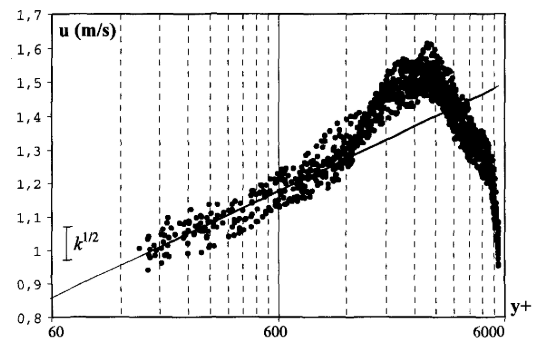
\includegraphics{Figures/research_papers/violeau2002-GLM-result.png}
    \caption{Turbulent Poiseuille flow in a pipe $(Re = 64e3)$ modelled using the generalised Langevin model. Computed mean velocity profiles after $(t=1s)$ (solid circles), against theory (solid line). Ref: \parencite{VIOLEAU2002}}
    \label{fig:violeau2002-GLM-result}
\end{figure}


\section{mSPH}
Adami et al. \parencite{Adami2012} devised a model built on their observation of SPH simulations, wherein the absence of viscosity in typical SPH formulations produced purely noisy particle motion. At finite viscosities, the method would over-predict dissipation. Hence to counter this, they essentially "modified" (hence the name: Modified SPH [mSPH]) the momentum equation and the equation of state to advect the particles in order to homogenise the particle distribution, in turn stabilising the numerical scheme. They were also able to reduce the artificial dissipation in transitional flows.

The authors considered summation density (\ref{eq:Adami2012-summation-density}), which is a function of the volume of the respective SPH particle as given by \ref{eq:Adami2012-vol}, as opposed to evolving density through the continuity equation \parencite{hu2006multi}. The modified equation of state as given by \ref{eq:Adami2012-eos}, is equivalent to the classical SPH equation-of-state with $\gamma=1$.
\begin{equation}
    \Vol_i = \frac{1}{\sum_j W_{ij}}
    \label{eq:Adami2012-vol}
\end{equation}
\begin{equation}
    \rho_i = \frac{m_i}{\Vol_i} = m_i\sum_j W_{ij}
    \label{eq:Adami2012-summation-density}
\end{equation}
\begin{equation}
    P_i = c_s^2 (\rho_i - \rho_0)
    \label{eq:Adami2012-eos}
\end{equation}

The momentum equation, which provides the acceleration of the particle, is a function of just the gradient and viscous shear forces as given by \ref{eq:Adami2012-mom-governing}. The corresponding SPH formulation was derived as given by \ref{eq:Adami2012-mom-sph}, which built on the earlier work of Hu and Adams \parencite{hu2007incompressible}.
\begin{equation}
    \LagDerivative{\vect{v}} = -\frac{1}{\rho}\nabla P + \nu \Delta \vect{v} 
    \label{eq:Adami2012-mom-governing}
\end{equation}
\begin{equation}
    \LagDerivative{\vect{v}_i} = -\frac{1}{m_i} \sum_j (\Vol^2_i + \Vol^2_j) \frac{P_i \rho_j + P_j \rho_i}{\rho_i + \rho_i} \DWIJ - \frac{\eta}{m_i} \sum_j (\Vol^2_i + \Vol^2_j) \frac{\VIJ}{\RtwoIJ[]}\DWIJ + \vect{F}_i
    \label{eq:Adami2012-mom-sph}
\end{equation}

This scheme takes advantage of the regularisation of the
particle motion stemming from the additional background pressure $(P_0 = \rho_0 c_s^2)$. The additional force exerted by the background pressure counteracts non-homogeneous particle distributions, therein reducing numerical dissipation.

The authors estimated the energy spectra of the flow simulations in order to analyse the results of their test cases, using first and second-order moving-least-squares (MLS) method \parencite{gossler2001moving} and its subsequent Fourier transform \parencite{frigo2005design}.
Their first test case, the $2D$ variant of the Taylor-Green Vortex (TGV) problem, involved $8\times 8$ counter-rotating vortices, requiring $64^2$ particles. They considered the viscosity to be zero.
As seen in the time evolution of the 
\begin{figure}[h]
    \centering
    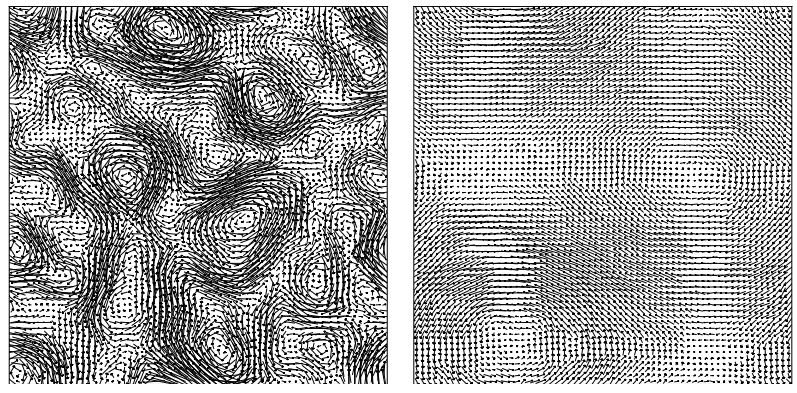
\includegraphics[scale=0.75]{Figures/research_papers/adami2012-evolution-vel-field-tgv.png}
    \caption{Velocity vector plot at $t=2$ (left) and $t=30$ (right). $Re = \infty$. Ref: \parencite{Adami2012} }
    \label{fig:adami2012-evolution-vel-field-tgv}
\end{figure}

The time evolution of the velocity field is given in \ref{fig:adami2012-evolution-vel-field-tgv}, where it can be observed that the $2D$ turbulence is characterised by merging and pairing of small vortices. The energy spectra given in \ref{fig:adami2012-energy-spectra-tgv} show that at low wave numbers, both interpolation schemes give the same results, but at high wave numbers, the results differ. The energy spectrum of the standard SPH has a linear slope of magnitude $m = 1$ in a log-log scale equivalent to a purely noisy velocity field. Theoretically, however, $2D$ turbulence has an energy cascade with a slope of $m = -3$ in the inertial range, which is reasonably predicted using mSPH.
\begin{figure}[h]
    \centering
    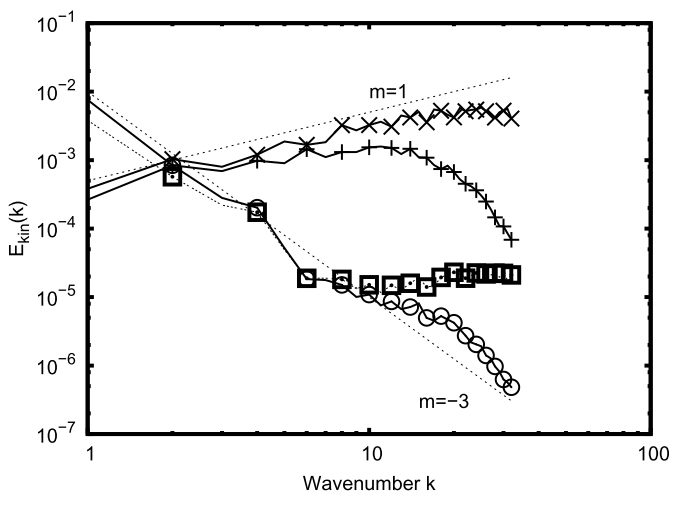
\includegraphics[scale=0.6]{Figures/research_papers/adami2012-energy-spectra-tgv.png}
    \caption{Comparison of energy spectra $t=10$. $+$ and $\times$ denote standard SPH results with quintic spline and MLS interpolation; $\circ$ and $\square$ denote mSPH results with quintic spline and MLS interpolation. Ref: \parencite{Adami2012} }
    \label{fig:adami2012-energy-spectra-tgv}
\end{figure}

The second test case employed by the authors was that of the $3D$ TGV problem requiring $64^3$ particles for a wide range of Reynolds numbers. The dissipation rate of the flow simulations are shown in \ref{fig:adami2012-dissipation-re400} and \ref{fig:adami2012-dissipation-re3000}. It can be observed that the standard SPH is unable to simulate transitional flows due to excessive dissipation. In contrast, mSPH can reproduce the dissipation rate reasonably well. This implies that the corrected particle transport velocity is an analogous eddy-viscosity model on scales below the numerical resolution.
\begin{figure}[h]
    \centering
    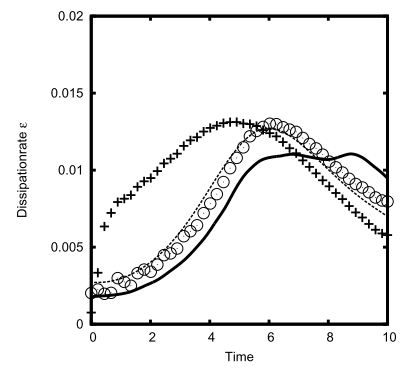
\includegraphics[scale=0.8]{Figures/research_papers/adami2012-dissipation-re400.png}
    \caption{Dissipation rate at $Re = 400$ using DNS (solid line), Smagorinsky model (dashed line), standard SPH ($+$) and mSPH ($\circ$). Ref: \parencite{Adami2012}}
    \label{fig:adami2012-dissipation-re400}
\end{figure}
\begin{figure}[h]
    \centering
    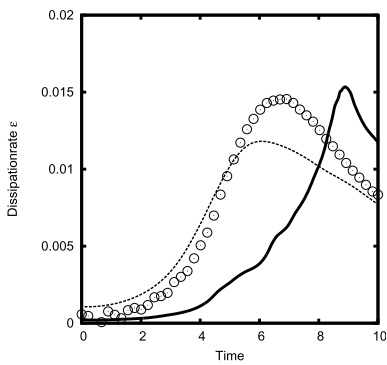
\includegraphics[scale=0.8]{Figures/research_papers/adami2012-dissipation-re3000.png}
    \caption{Dissipation rate at $Re = 3000$ using DNS (solid line), Smagorinsky model (dashed line) and mSPH ($\circ$). Ref: \parencite{Adami2012}}
    \label{fig:adami2012-dissipation-re3000}
\end{figure}

\section{Large Eddy Simulation-based Models}
\subsection{Implicit Pressure Poisson-based Solvers}

\subsection{Explicit Pressure Equation of State-based Solvers}
Weakly compressible solvers